\section{Zielsetzung}
\label{sec:zielsetzung}

    In diesem Versuch soll das Experiment, in welchem die Physiker James Franck und Gustav Hertz im Jahr 1914 die Energieübertragung bei Stößen von Elektronen mit 
    Atomen untersucht haben, näher betrachtet werden. Dazu wird der Versuchsaufbau nachempfunden und die Messungen der Physiker wiederholt. Es wird die 
    Energiedifferenz zwischen dem ersten angeregten Zustand und dem Grundzustand, die Energieverteilung der Elektronen und die Ionisationsenergie des 
    Quecksilberatoms ermittelt werden. 

\section{Theorie}
\label{sec:Theorie}

    Der Franck-Hertz-Versuch gehört zu einer dreijährigen Messreihe der Physiker James Franck und Gustav Hertz. In dem Elektronenstoßexperiment gelingt es einer
    Anregungsenergie des Quersilberatoms zu ermitteln und einen Zusammenhang von dieser mit der Wellenlänge des Photons, welches beim Zurückgehen in den 
    Grundzustand emittiert wird, aufzustellen. Damit können im gewissen Maße die Bohr'schen Postulate, welche 1913 von Niels Bohr aufgestellt wurden, experimentell verifiziert 
    werden und die Elektronenhülle besser verstanden werden. \\
    
    \noindent Bei einem Elektronenstoßexperiment werden Atome mit Elektronen beschossen und aus den Energiedifferenzen der Elektronen Rückschlüsse gezogen. 
    In dem Franck-Hertz-Versuch werden Quecksilberatome mit Elektronen verschiedener Energien beschossen und stoßen elastisch und inelastisch miteinander. 


\subsection{Aufbau und Ablauf des Franck-Hertz-Versuches}

    In der \autoref{fig:prinzipieller_aufbau} ist die Franck-Hertz-Apparatur schematisch dargestellt. Ihr Hauptteil ist ein evakuiertes Gefäß, in welchem ein 
    Tropfen Quecksilber ist. Dadurch entsteht ein Gleichgewichtsdruck, der sich entlang der Dampfdruckkurve entwickelt und steuerbar nur über die Temperatur ist. 
    Mithilfe des glühelektrischen Effekts werden die Elektronen am Glühdraht ausgelöst, an welchem eine Gleichspannung anliegt. Um die Anzahl an ausgelösten 
    Elektronen zu vergrößern, wird häufig der Glühdraht mit einem Material mit geringer Auslösungsenergie bestrichen. 

    \begin{figure}
         \centering 
         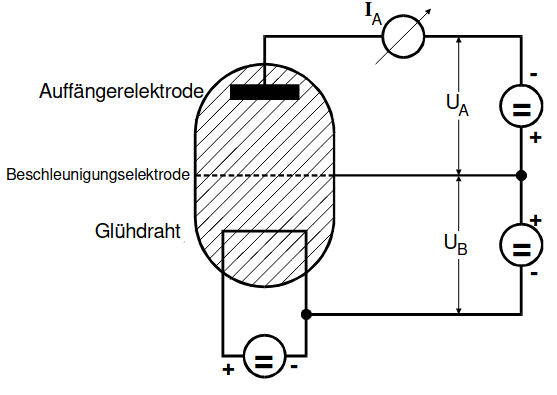
\includegraphics[width=0.6\textwidth]{bilder/prinzipieller_aufbau.png}
         \caption{Prinzipieller Aufbau des Franck-Hertz-Versuches \cite{anleitung}.}
         \label{fig:prinzipieller_aufbau}
    \end{figure}

    \noindent In dem Gefäß ist ein Gitter, zwischen diesem und dem Glühdraht wird eine Beschleunigungsspannung gelegt. Die Elektronen bekommen durch das 
    Durchlaufen dieser Spannung die Energie 
    \begin{equation*}
        \frac{m_0 v^2_{\text{vor}}}{2} = e_0 \cdot U_{\text{B}}. 
    \end{equation*}
    Aus dieser lässt sich eine Geschwindigkeit für die Elektronen nach Durchlaufen der Beschleunigungsspannung angeben, es wird der Fall betrachtet, dass die
    Elektronen vorher keine Geschwindigkeit haben. \\
    Zwischen dem Gitter und der Auffängerelektrode liegt wiederum eine Spannung, welche jedoch andersherum gepolt ist, also ein Gegenfeld für die Elektronen darstellt. 
    Somit gilt für die an der Auffängerelektrode ankommenden Elektronen
    \begin{equation*}
        \frac{m_0}{2} v_{\text{z}}^2 \geq e_0 U_{\text{A}}. 
    \end{equation*}
    Der Strom kann mit einem Amperemeter  gemessen werden. 

    \noindent Die Elektronen können mit den Quecksilberatomen elastische und inelastische Stöße durchführen. Elastische Stöße treten auf, wenn die Energie der Elektronen 
    gering ist. Die Energieabgabe des Elektrons an das Hg-Atom beträgt im zentralen Stoß etwa
    \begin{equation*}
        \increment E = \frac{4 m_0 M}{(m_0 + M)^2}E \approx \num{1.1e-5}E \, . 
    \end{equation*}
    Diese ist also vernachlässigbar klein, jedoch sollte die Richtungsänderung des Elektrons durch den Stoß weiterhin beachtet werden, da dadurch manche Elektronen das 
    Gegenfeld nicht mehr durchlaufen können. \\
    Besitzt das Elektron eine Energie $E \geq E_1 - E_0 $, also eine Energie, die größer oder gleich der Energiedifferenz des ersten angeregtem Zustand und des Grundzustand 
    ist, so kann durch einen Stoß ein Hg-Atom angeregt werden. Dabei wird diese Energiedifferenz an die Elektronenhülle übertragen, das Elektron behält die restliche
    Energie. Nach einer Relaxationszeit von $\SI{1e-8}{\second}$ geht das angeregte Quecksilberatom durch Emission eines Lichtquant der Energie 
    \begin{equation*}
        E = \symup{h} \nu = E_1 - E_0
    \end{equation*}
    wieder in den Grundzustand zurück. Durch das Anregen der Atome geben die Elektronen einen Teil ihrer Energie ab, sodass beim Auftreten von inelastischen Stößen viele Elektronen
    das Gegenfeld nicht mehr durchlaufen können. Der gemessene Auffängerstrom nimmt sehr plötzlich ab. Wird die Beschleunigungsspannung erhöht, so haben die Elektronen nach durchlaufen
    des Feldes wieder genug Energie um gegen das Gegenfeld anzukommen, der Auffängerstrom steigt wieder. Beim weiteren Erhöhen der Beschleunigungsspannung bekommen die Elektronen 
    nach dem ersten Anregen eines Atoms genug Energie, um ein weiteres Atom anzuregen, sodass der Auffängerstrom wieder abfällt. Dieser ideale Verlauf der Franck-Hertz-Kurve ist in 
    der \autoref{fig:idealisiert} zu sehen. 

    \begin{figure}[H]
        \centering 
        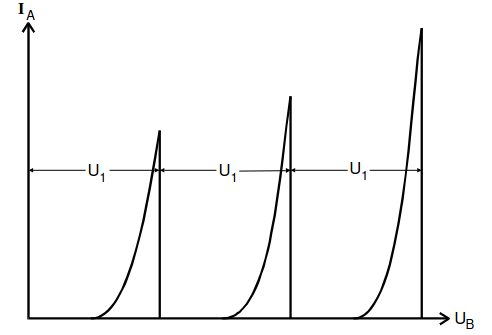
\includegraphics[width=0.6\textwidth]{bilder/idealer_Ub_Ia.png}
        \caption{Idealisierter Zusammenhang zwischen dem Strom des Gegenfeldes $I_{\text{A}}$ und der Beschleunigungsspannung $U_{\text{B}}$ \cite{anleitung}. }
        \label{fig:idealisiert}
    \end{figure}

    \noindent Für den Abstand zweier benachbarter Maxima gilt der Zusammenhang:
    \begin{equation*}
        U_1 = \frac{1}{e_0} \left( E_1 - E_0 \right)
    \end{equation*}
    Dies entspricht, wie die obigen Überlegungen auch fordern, der Energiedifferenz des ersten angeregten Zustands und des Grundzustand des Quecksilberatom. 

\subsection{Einflüsse auf die Gestalt der Franck-Hertz-Kurve}

    Die real messbare Franck-Hertz Kurve sieht leicht anders aus als der idealisierte Verlauf, welcher in der \autoref{fig:idealisiert} zu sehen ist. 
    Dies folgt aus einigen Nebeneffekten. 

    \subsubsection{Einfluss des Kontaktpotentials}

        Damit bereits bei geringen Temperaturen eine hohe Anzahl an Elektronen aus der Glühkathode gelöst werden kann, wird diese oft mit einem Material mit 
        kleiner Austrittarbeit bestrichen. Besonders wichtig ist es, dass das Material eine geringere Austrittsarbeit $\Phi_{\text{G}}$ als das Material der Beschleunigungselektrode $\Phi_{\text{B}}$ 
        hat, sodass die Elektronen aus der Glühkathode ausgelöst werden und nicht aus der Beschleunigungselektrode. Dadurch ist das wahre Beschleunigungspotential 
        verschieden von der angelegten Spannung $U_{\text{B}}$. Die Potentialverhältnisse sind in der \autoref{fig:potentialberhaltnis} aufgezeichnet; 
        es gilt für das wirkliche Beschleunigungspotential:
        \begin{equation*}
            U_{\text{B, eff}} = U_{\text{B}} - \frac{1}{e_0} \left( \Phi_{\text{B}} - \Phi_{\text{G}} \right)
        \end{equation*}
        Die Franck-Hertz-Kurve ist im wahren Experiment um den Wert $K \coloneq \frac{1}{e_0} \left( \Phi_{\text{B}} - \Phi_{\text{G}} \right)$ verschoben, dieser 
        Ausdruck wird auch Kontaktpotential genannt. 

        \begin{figure}[H]
            \centering 
            \includegraphics[width=0.7\textwidth]{bilder/Potentialverhältnisse.png}
            \caption{Potentialverhältnisse zwischen Glühkathode und Beschleunigungselektrode \cite{anleitung}.}
            \label{fig:potentialberhaltnis}
        \end{figure}


    \subsubsection{Einfluss des Energie-Spektrums der Elektronen}

        Elektronen haben im Inneren eines Metalls bereits ein Energie-Spektrum, dieses ist als Fermi-Dirac-Verteilung bekannt. Dadurch ist ihre Energie nach 
        Durchlaufen der Beschleunigungsspannung auch durch eine Energieverteilung gegeben, sie fängt bei $U_{\text{B, eff}}$ an und steigt kontinuierlich, bei 
        höher werdenen Energien nimmt die Häufigkeit jedoch schnell ab. Dies bedeutet für die Franck-Hertz-Kurve, dass die Steigung beim Annähern an ein Maximum 
        verringert ist und die Kurve sich im Abfall stetig einem Stromminimum nähert. \\

        \noindent Außerdem haben die oben angesprochenen elastischen Stöße einen Einfluss auf die Kurve. Elastische Stöße, bei welchen die Richtung der Elektronen 
        geändert wird, machen keinen zu großen Unterschied, solange sie zwischen Glühkathode und Beschleunigungselektrode ablaufen, da sie dort durch die 
        Beschleunigungsspannung wieder in die richtige Richtung gelenkt werden. Führen die Elektronen jedoch in dem Raum zwischen Beschleunigungseletrode und 
        Auffängerkathode elastische Stöße mit den Quecksilberatomen aus, so können diese eine Richtungsänderung in der für das Gegenfeld relevante Komponente 
        bekommen und so das Gegenfeld nicht komplett durchlaufen. Dadurch wird die Franck-Hertz Kurve verbreitert und abgeflacht. 

    \subsubsection{Einfluss des Dampfdruckes}

        Damit es zu genügend Stößen zwischen Elektronen und Quecksilberatomen kommt, muss die mittlere freie Weglänge der Atome $\bar{w}$ klein gegen den Abstand zwischen 
        Glühkathode und Beschleunigungselektrode sein. Aus der kinetischen Gastheorie folgt der Zusammenhang
        \begin{equation*}
            \bar{w} = \frac{0,0029}{p_{\text{sät}}}, 
        \end{equation*}
        wobei die mittlere freie Weglänge $\bar{w}$ hier in $\si{\centi\metre}$ gegeben ist und der Sättigungsdampfdruck $p_{\text{sät}}$ in $\si{\milli\bar}$. 
        Aus der Dampfdruckkurve ist der Sättigungsdampfdruck in Abhängigkeit der Temperatur abzulesen, in der \autoref{fig:dampfdruckkurve} ist dies für 
        Quecksilber aufgezeichnet. Es gilt die Formel 
        \begin{equation*}
            p_{\text{sät}}(T) = 5,5 \cdot 10^7 \exp(\frac{-6876}{T}), 
        \end{equation*}
        wobei der Sättigungsdampfdruck $p_{\text{sät}}$ in $\si{\milli\bar}$ und die Temperatur $T$ in $\si{\kelvin}$ gegeben ist. 

        \begin{figure}[H]
            \centering 
            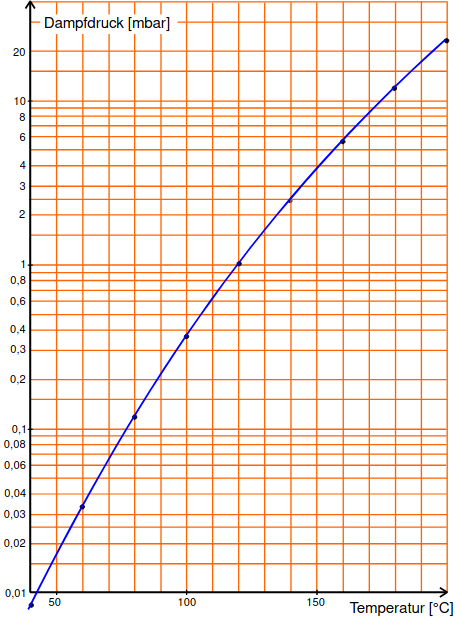
\includegraphics[width=0.7\textwidth]{bilder/Dampfdruckkurve.png}
            \caption{Dampfdruckkurve des Quecksilbers \cite{anleitung}.}
            \label{fig:dampfdruckkurve}
        \end{figure}

        \noindent Somit gibt es einen Dampfdruckbereich, also Temperaturbereich, in dem die Franck-Hertz-Apparatur gut arbeitet. Ein zu geringer Dampfdruck sorgt
        dafür, dass Elektronen das Beschleunigungspotential durchlaufen ohne einen Stoß zu haben. Dies ist einerseits nicht zielführend, da keine inelastischen Stöße 
        ausgeführt werden, welche für den Versuch essentiell sind, andererseits können die Elektronen somit auch vor einem seltenen Stoß genügend Energie aufnehmen, 
        dass sie in der Lage sind das Quecksilberatom auch auf ein höheres Energieniveau zu heben. Ein zu hoher Dampfdruck sorgt dafür, dass viele elastische Stöße 
        ausgeführt werden und somit die Anzahl der Elektronen, welchen an der Auffängerelektrode ankommen, abnimmt. 


\subsection{Aufbau der Hg-Elektronenhülle}

    Aufgrund des Aufbaus der Elektronenhülle von Quecksilber gehen die Elektronen nicht aus dem Grundzustand von n=6, S=0 und L=0 in den energetisch höheren 
    Zustand n=7, S=0, L=0 über. Hierfür müsste der Elektronenspin umklappen, was sehr unwahrscheinlich ist. Im Franck-Hertz-Versuch erfolgt die Anregung des 
    Triplett-Zustandes aus dem Singulett-Zustand, da das stoßende Elektron gegen eines der 6s-Elektronen mit entgegengesetztem Spin ausgetauscht wird. 
    Diese beobachtete und die theoretische Energierelation ist in einem Termschema in der \autoref{fig:termschema} abgebildet. 
    
    \begin{figure}[H]
        \centering 
        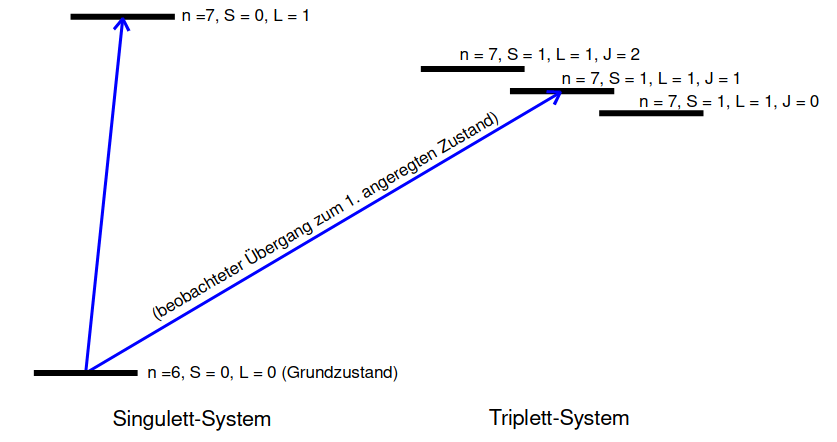
\includegraphics[width=0.8\textwidth]{bilder/Termschema.png}
        \caption{Ein nicht maßstäbliches Termschema eines Hg-Atoms \cite{anleitung}.}
        \label{fig:termschema}
    \end{figure}

    % \noindent Die tatsächliche Energie des Übergangs wird dadurch verringert, dass das Umklappen des Elektronenspins sehr 
    % unwahrscheinich ist. Aus dem Grundzustand von n=6, S=0 und L=0 übergeht das Elektronen also nicht in den höher energetischen 
    % Zustand n=7, S=0, L=0 des Singluett-System. Beobachtet wird der Übergang in einer der Zustäde des Triplett-Systems, diese sind in 
    % Abbildung(\ref{img:Term}) zu sehen. Diese Stöße sind wahrscheinlicher da das Stoßelektron gegen einer der 6s Elektronen mit 
    % entgegengesetztem Spin ausgetauscht wird.

